\documentclass[12pt,a4paper,openany]{book}
\usepackage{lmodern}
\usepackage[svgnames]{xcolor} % Required to specify font color
\input{../LaTexTemplate/templates/couleurs.tex}

\usepackage{makeidx}
\usepackage[utf8]{inputenc} 
\usepackage{marvosym}
\usepackage[T1]{fontenc}
\usepackage[francais]{babel}
\usepackage[top=1.7cm, bottom=1.7cm, left=1.7cm, right=1.7cm]{geometry}
\usepackage{verbatim}
\usepackage[urlbordercolor={1 1 1}, linkbordercolor={1 1 1}, linkcolor=vert1, urlcolor=bleu, colorlinks=true]{hyperref}
\usepackage{tikz} %Vectoriel
\usepackage{listings}
\usepackage{fancyhdr}
\usepackage{multido}
\usepackage{amssymb}
\usepackage{slashbox}
\usepackage{float}
\usepackage[francais]{minitoc}
\usepackage[final]{pdfpages} 
\usepackage{pgfgantt}
\usepackage{graphicx} % Required for box manipulation
\usepackage{makeidx}
\usepackage{lscape}
\usepackage{rotating}
\usepackage{epstopdf}


\newcommand{\titre}{Maison Intelligente}
%\newcommand{\logoFooter}{\begin{minipage}{0.1\textwidth}\includegraphics[width=2cm]{../../images/FACT_official.png}\end{minipage}}
\newcommand{\titreFooter}{Maison Intelligente} 
\newcommand{\subtitle}{Salle de bain} 
\newcommand{\auteur}{}
\newcommand{\semestre}{}
\newcommand{\annee}{2016}


\newcommand{\pole}{}
\newcommand{\sigle}{}
\newcommand{\FactDev}{\textit{FactDev}}
\newcommand{\key}[1]{\textit{#1}}
\newcommand{\approved}{true}

\makeindex
\usepackage[totoc]{idxlayout}


\input{../LaTexTemplate/templates/listings.tex}
\input{../LaTexTemplate/templates/classroomsTemplates/l3/cours.tex}
\input{../LaTexTemplate/templates/remarquesExempleAttention.tex}
\input{../LaTexTemplate/templates/polices.tex}
\input{../LaTexTemplate/templates/affichageChapitre.tex}


\newcommand*{\plogo}{\fbox{$\mathcal{PL}$}} % Generic publisher logo
%----------------------------------------------------------------------------------------
%	TITLE PAGE
%----------------------------------------------------------------------------------------

\newcommand*{\rotrt}[1]{\rotatebox{90}{#1}} % Command to rotate right 90 degrees
\newcommand*{\rotlft}[1]{\rotatebox{-90}{#1}} % Command to rotate left 90 degrees

\newcommand*{\titleBC}{\begingroup % Create the command for including the title page in the document
\newlength{\drop} % Command for generating a specific amount of whitespace
\drop=0.1\textheight % Define the command as 10% of the total text height

\vspace*{-50px}
\rule{\textwidth}{0.4pt}\par % Thick horizontal line
\begin{tabular}{p{8cm}p{5cm}p{6cm}}
	\begin{minipage}{8cm}
		Florent \bsc{Berbie}\\
		Antoine de \bsc{Roquemaurel}\\~\\
		
\includegraphics[width=5cm]{mdl.png}
	\end{minipage} &
	& 

	\begin{minipage}{5cm}
		\begin{center}
			
\includegraphics[width=5cm]{logo.jpg}\\
			\tiny{Rédigé avec \LaTeX{}\\Version du \today}
		\end{center}
	\end{minipage}
\end{tabular}


\vspace{\drop} % Whitespace between the top lines and title
\centering % Center all text

\vspace{100px}
\def\CP{\textit{\Huge \titre}} % Title

\settowidth{\unitlength}{\CP} % Set the width of the curly brackets to the width of the title
{\color{LightGoldenrod}\resizebox*{\unitlength}{\baselineskip}{\rotrt{$\}$}}} \\[\baselineskip] % Print top curly bracket
\textcolor{Sienna}{\CP} \\[\baselineskip] % Print title
{\color{RosyBrown}\Large \subtitle} \\ % Tagline or further description
{\color{LightGoldenrod}\resizebox*{\unitlength}{\baselineskip}{\rotlft{$\}$}}} % Print bottom curly bracket

\vfill % Whitespace between the title and the author name


{
\normalsize \LARGE Université Toulouse III -- Paul Sabatier}\\ % Author name

\vfill % Whitespace between the author name and the publisher logo
\Large \today % Year published

\rule{\textwidth}{0.4pt}\par % Thick horizontal line

\endgroup}

%----------------------------------------------------------------------------------------
%	BLANK DOCUMENT
%----------------------------------------------------------------------------------------


\makeatother
\includeonly {
	contents/0_introduction,
	contents/1_diagram_exigences,
	contents/2_diagram_use_case,
	contents/3_diagram_blocks_bdd,
	contents/4_diagram_blocks_ibd,
	contents/5_diagramme_states,
	contents/6_diagram_sequences
}
\begin{document}
	\thispagestyle{empty} % Removes page numbers
%	\titleBC
	\dominitoc
	\setcounter{tocdepth}{1}
	\setcounter{secnumdepth}{3}
	\setcounter{minitocdepth}{1}
	
	\tableofcontents

	% Introcution #1 -----------------------
	\chapter*{À propos}

La \textbf{Maison Intelligente} (MI) constitue un lieu où technologies et sciences humaines se rencontrent pour trouver des solutions permettant d'aider à l'accompagnement du vieillissement des populations dans notre société (handicaps, dépendances, etc).
 
Pour ce faire, la Maison Intelligente propose un ensemble de solutions permettant à celle-ci de s'adapter à son habitant.  L'ensemble des possibilités qu'offre la MI sont définies dans le document : M2DL2015-ExigencesMI.
% (cf. https://docs.google.com/spreadsheets/d/1-yaW8fZHG9i6r7vJ7NOU9-66-hnDYY66Vd9cmZTYs2A/edit ). 


L'objectif du document est de proposer un ensemble de diagrammes définies au moyen de la norme SysML répondant aux exigences relatives à la \textbf{salle de bain} de la MI.

Les diagrammes ici représentés seront :
\begin{itemize}
	\item diagramme des \textbf{exigences} (req)
	\item diagramme des \textbf{cas d'utilisation} (uc)
	\item diagramme de \textbf{blocs de définition} (bdd)
	\item diagramme \textbf{interne de blocs} (idb)
	\item diagramme comportementaux
	\begin{itemize}
		\item diagramme d'\textbf{états} (st)
		\item diagramme de \textbf{séquences} (seq)
	\end{itemize}
\end{itemize} 		
	
	\chapter{Diagramme des exigences (req)}\label{req}
Les exigences de la salle de bain sont réparties en plusieurs parties, et concernent l'adaptation de celle-ci à l'habitant : 
\begin{itemize}
	\item L'adaptation des meubles
	\item L'adaptation de l'éclairage
	\item L'adaptation de la température de la pièce
\end{itemize}
\begin{figure}[H]
	\centering
	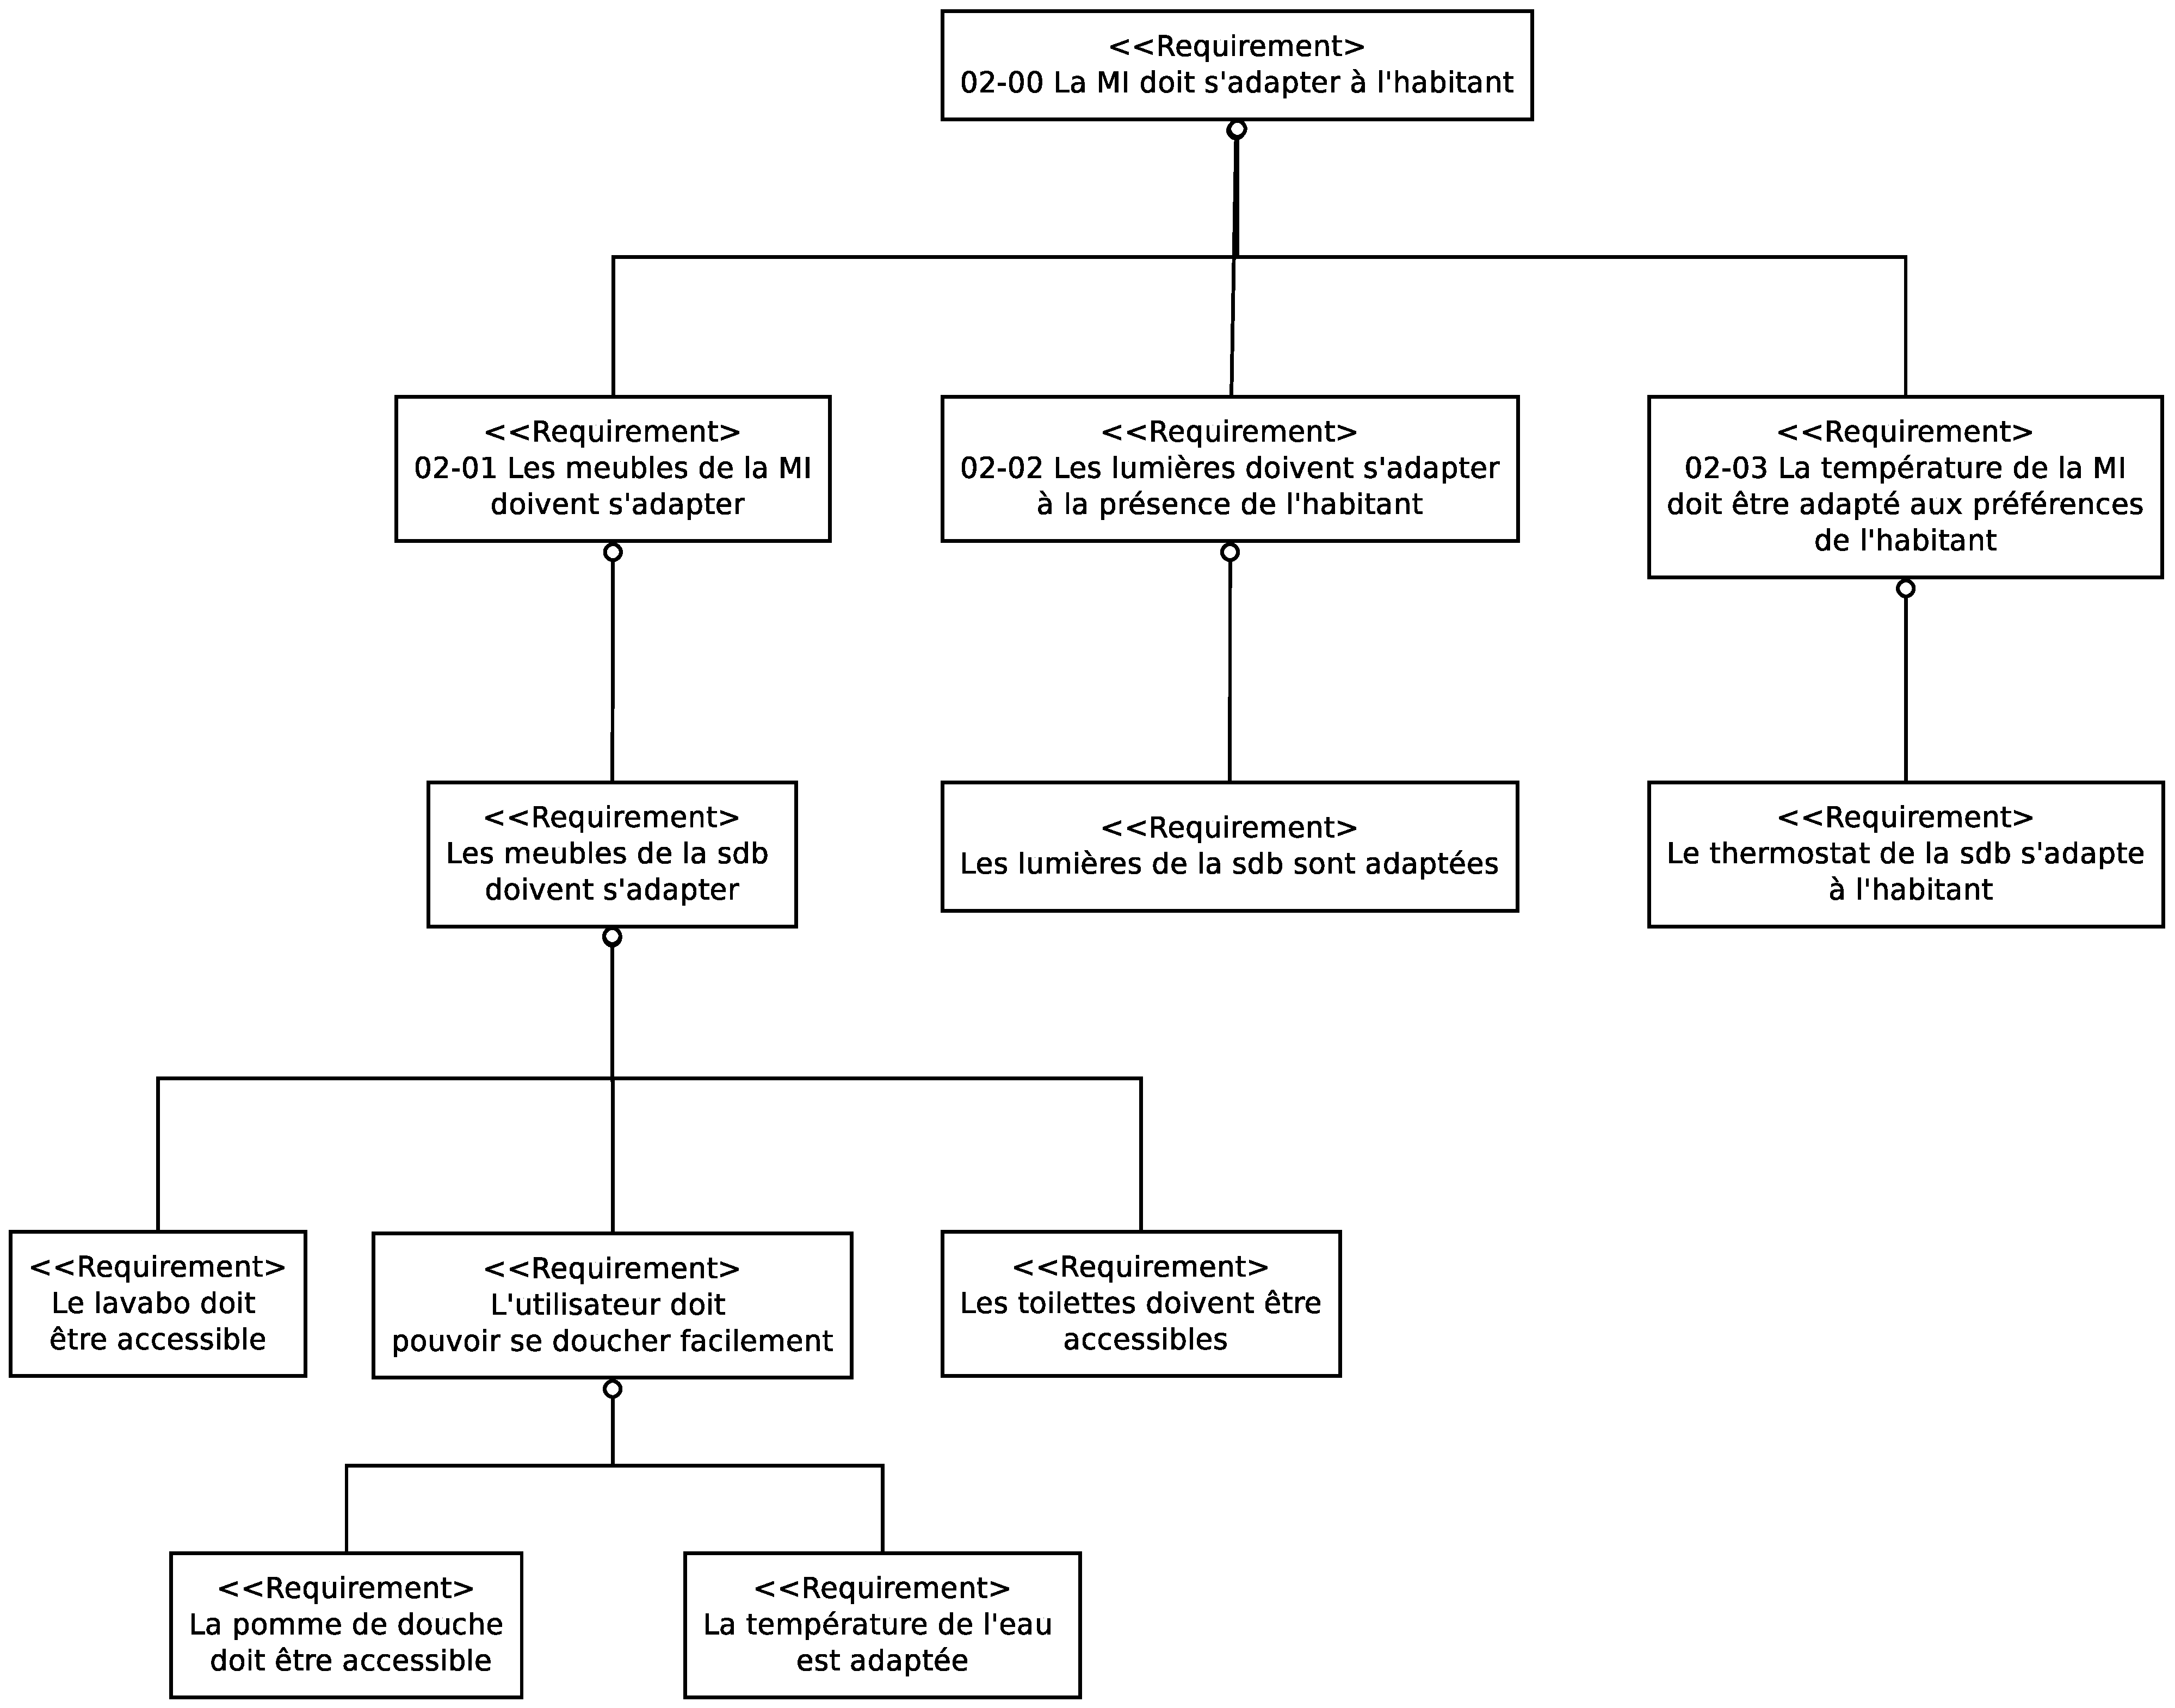
\includegraphics[width=1\linewidth]{diagrams/bathroom/diagramme_exiquences_req.eps}
	\caption{Diagramme de bloc de définition}
	\label{fig:requirements}
\end{figure}
 % Diagramme des exigences #2	
	\chapter{Diagramme des cas d'utilisations}
  % Diagramme des cas d'utilisation #3
	\chapter{Diagrammes de blocs de définition}
\section{Diagramme de blocs général}
Afin de répondre à l'ensemble des exigences présentées section \ref{req}, figure \ref{fig:requirements}, la salle de bain possède différents blocks : 
\begin{description}
	\item[Mobilier] Concerne les équipements devant s'adapter à l'habitant
	\item[Eclairage] Tout ce qui est prévu pour l'adaptation de l'éclairage 
	\item[Radiateurs] L'adaptation de la température de la pièce
	\item[Contrôleur] Un système permettant de contrôler les éléments de notre salle de bain. Ce système contient un micro-contrôleur permettant l'utilisation des capteurs et actionneurs, un système de
		communication avec les données de la maison intelligente, ainsi qu'un logiciel effectuant les traitements nécessaires (monter/descendre un mobilier, augmenter la température de la pièce,
		\ldots)
\end{description}

\begin{figure}[H]
	\centering
	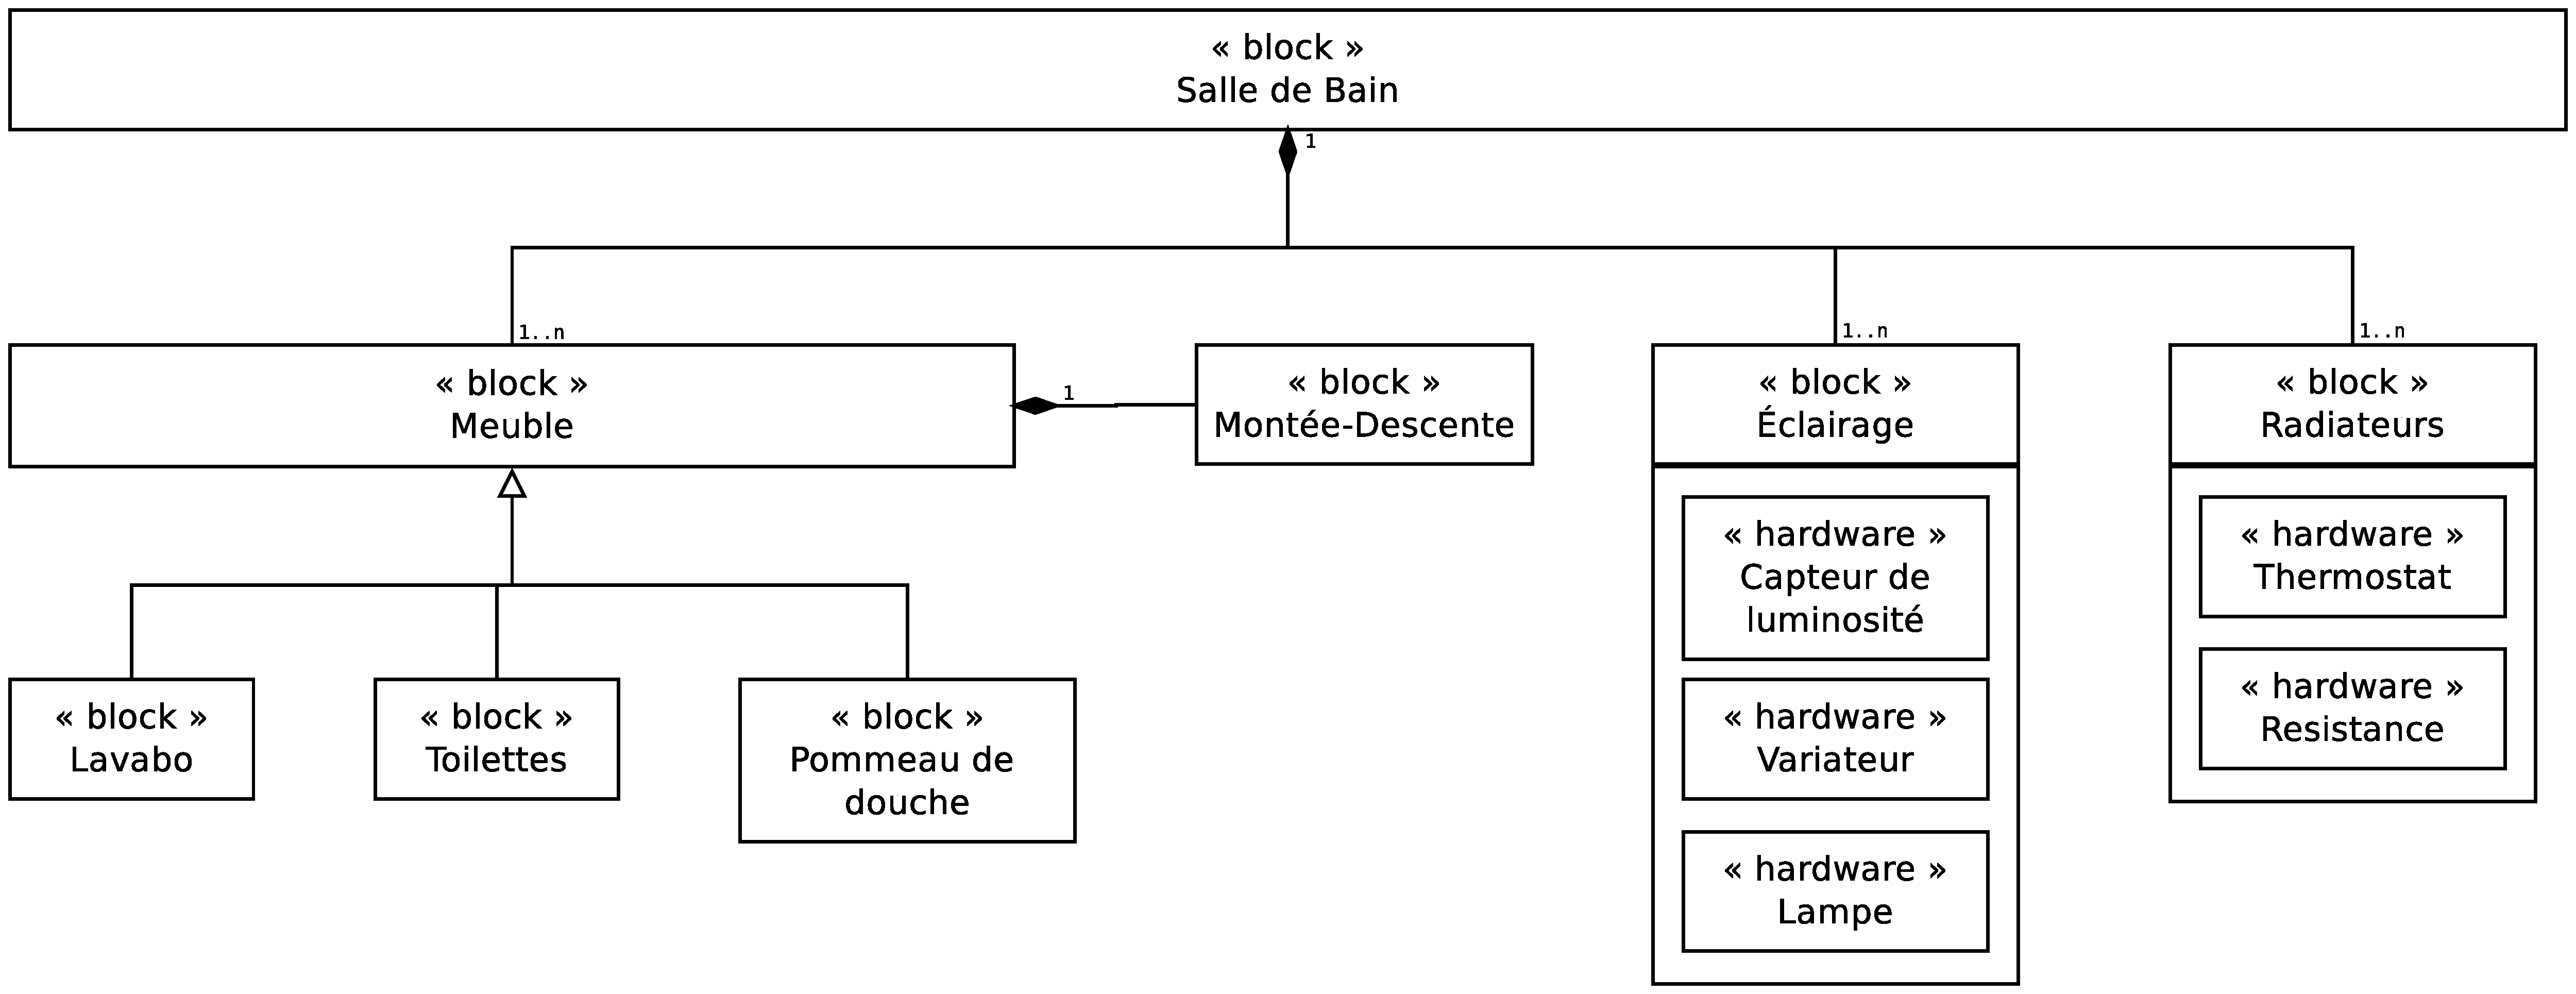
\includegraphics[width=1\linewidth]{diagrams/bathroom/diagramme_blocks_bdd.eps}
	\caption{Diagramme de bloc de définition}
	\label{fig:diagramme_bdd}
\end{figure}

\section{Diagramme de bloc de « Montée-Descente »}
Chaque mobilier doit pouvoir moduler sa hauteur pour s'adapter à l'habitant de la MI. Chaque mobilier de la salle de bain est doté d'un bloc « Montée-Descente » comportant :
\begin{description}
	\item[Capteur de mouvement Infra-Rouge] détermine les mouvements de l'habitant
	\item[Capteur laser] permet de déterminer la taille de l'habitant afin de pouvoir s'adapter à lui
	\item[Système élévateur] permet de monter ou descendre la dalle supportant le mobilier (ou l'habitant si celui-ci est dans la douche) en fonction de sa position actuelle et de la taille de l'habitant.   
\end{description}

\begin{figure}[H]
	\centering
	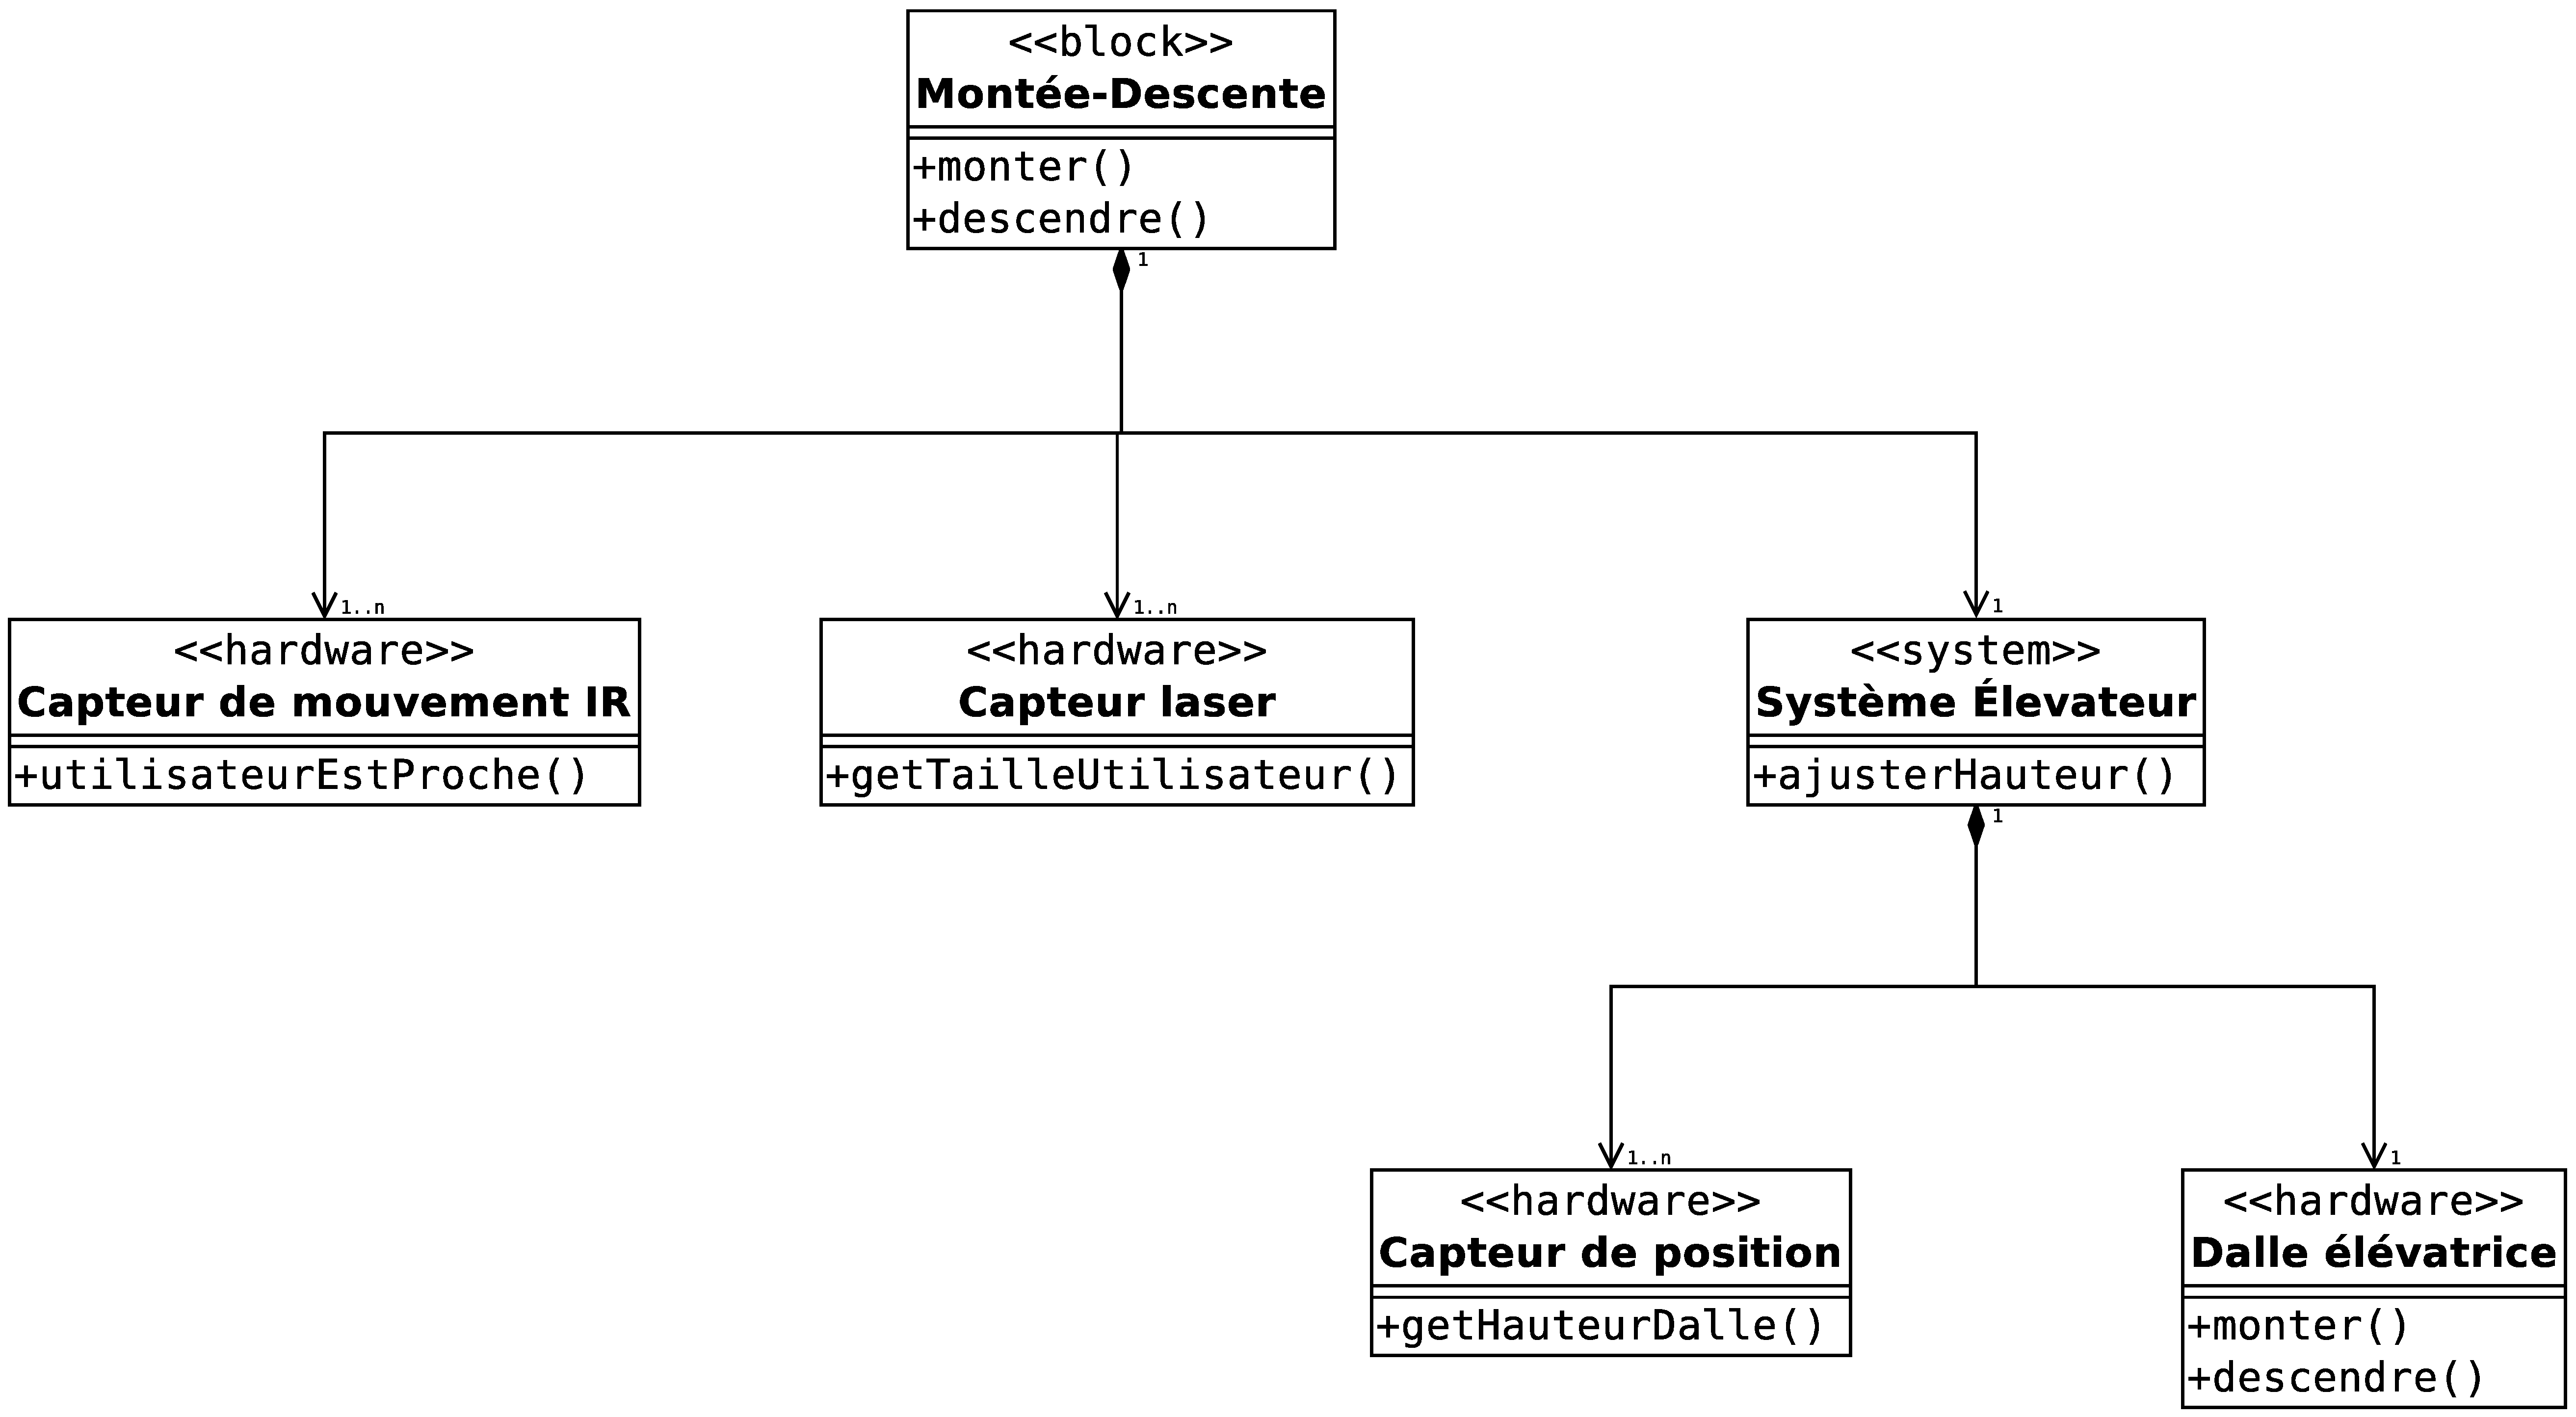
\includegraphics[width=1\linewidth]{diagrams/bathroom/diagramme_blocks_bdd2.eps}
	\caption{Diagramme de bloc de définition de « Montée-Descente »}
	\label{fig:diagramme_bdd2}
\end{figure}
 % Diagrammes de blocks (bdd) #4	
	\chapter{Diagrammes internes de blocs (ibd)}
Le \textbf{Système élévateur} associé aux meubles permettant d'adapter la hauteurs de ces derniers à celle de l'habitant fonctionne de la façon présentée ci-dessous.

Nous prenons ici le cas de la douche.

Le système reçoit deux paramètres: la hauteur de l'habitant \textbf{\textit{hauteurHabitant}} (nulle si personne est dans la douche) et une valeur booléenne \textbf{\textit{estDansLaDouche}}indiquant si l'utilisateur se trouve dans la douche. 
La hauteur de l'habitant est transmise au \textbf{Contrôleur} qui va à son tour récupérer la position du mobilier, c'est-à-dire sa hauteur \textbf{\textit{hauteurMobilier}} par rapport au sol. Il va comparer cette valeur obtenue à la hauteur de l'habitant récupérée en entrée afin de déterminer la position de la dalle élévatrice \textbf{\textit{positionDalle}}. 
\begin{figure}[H]
	\centering
	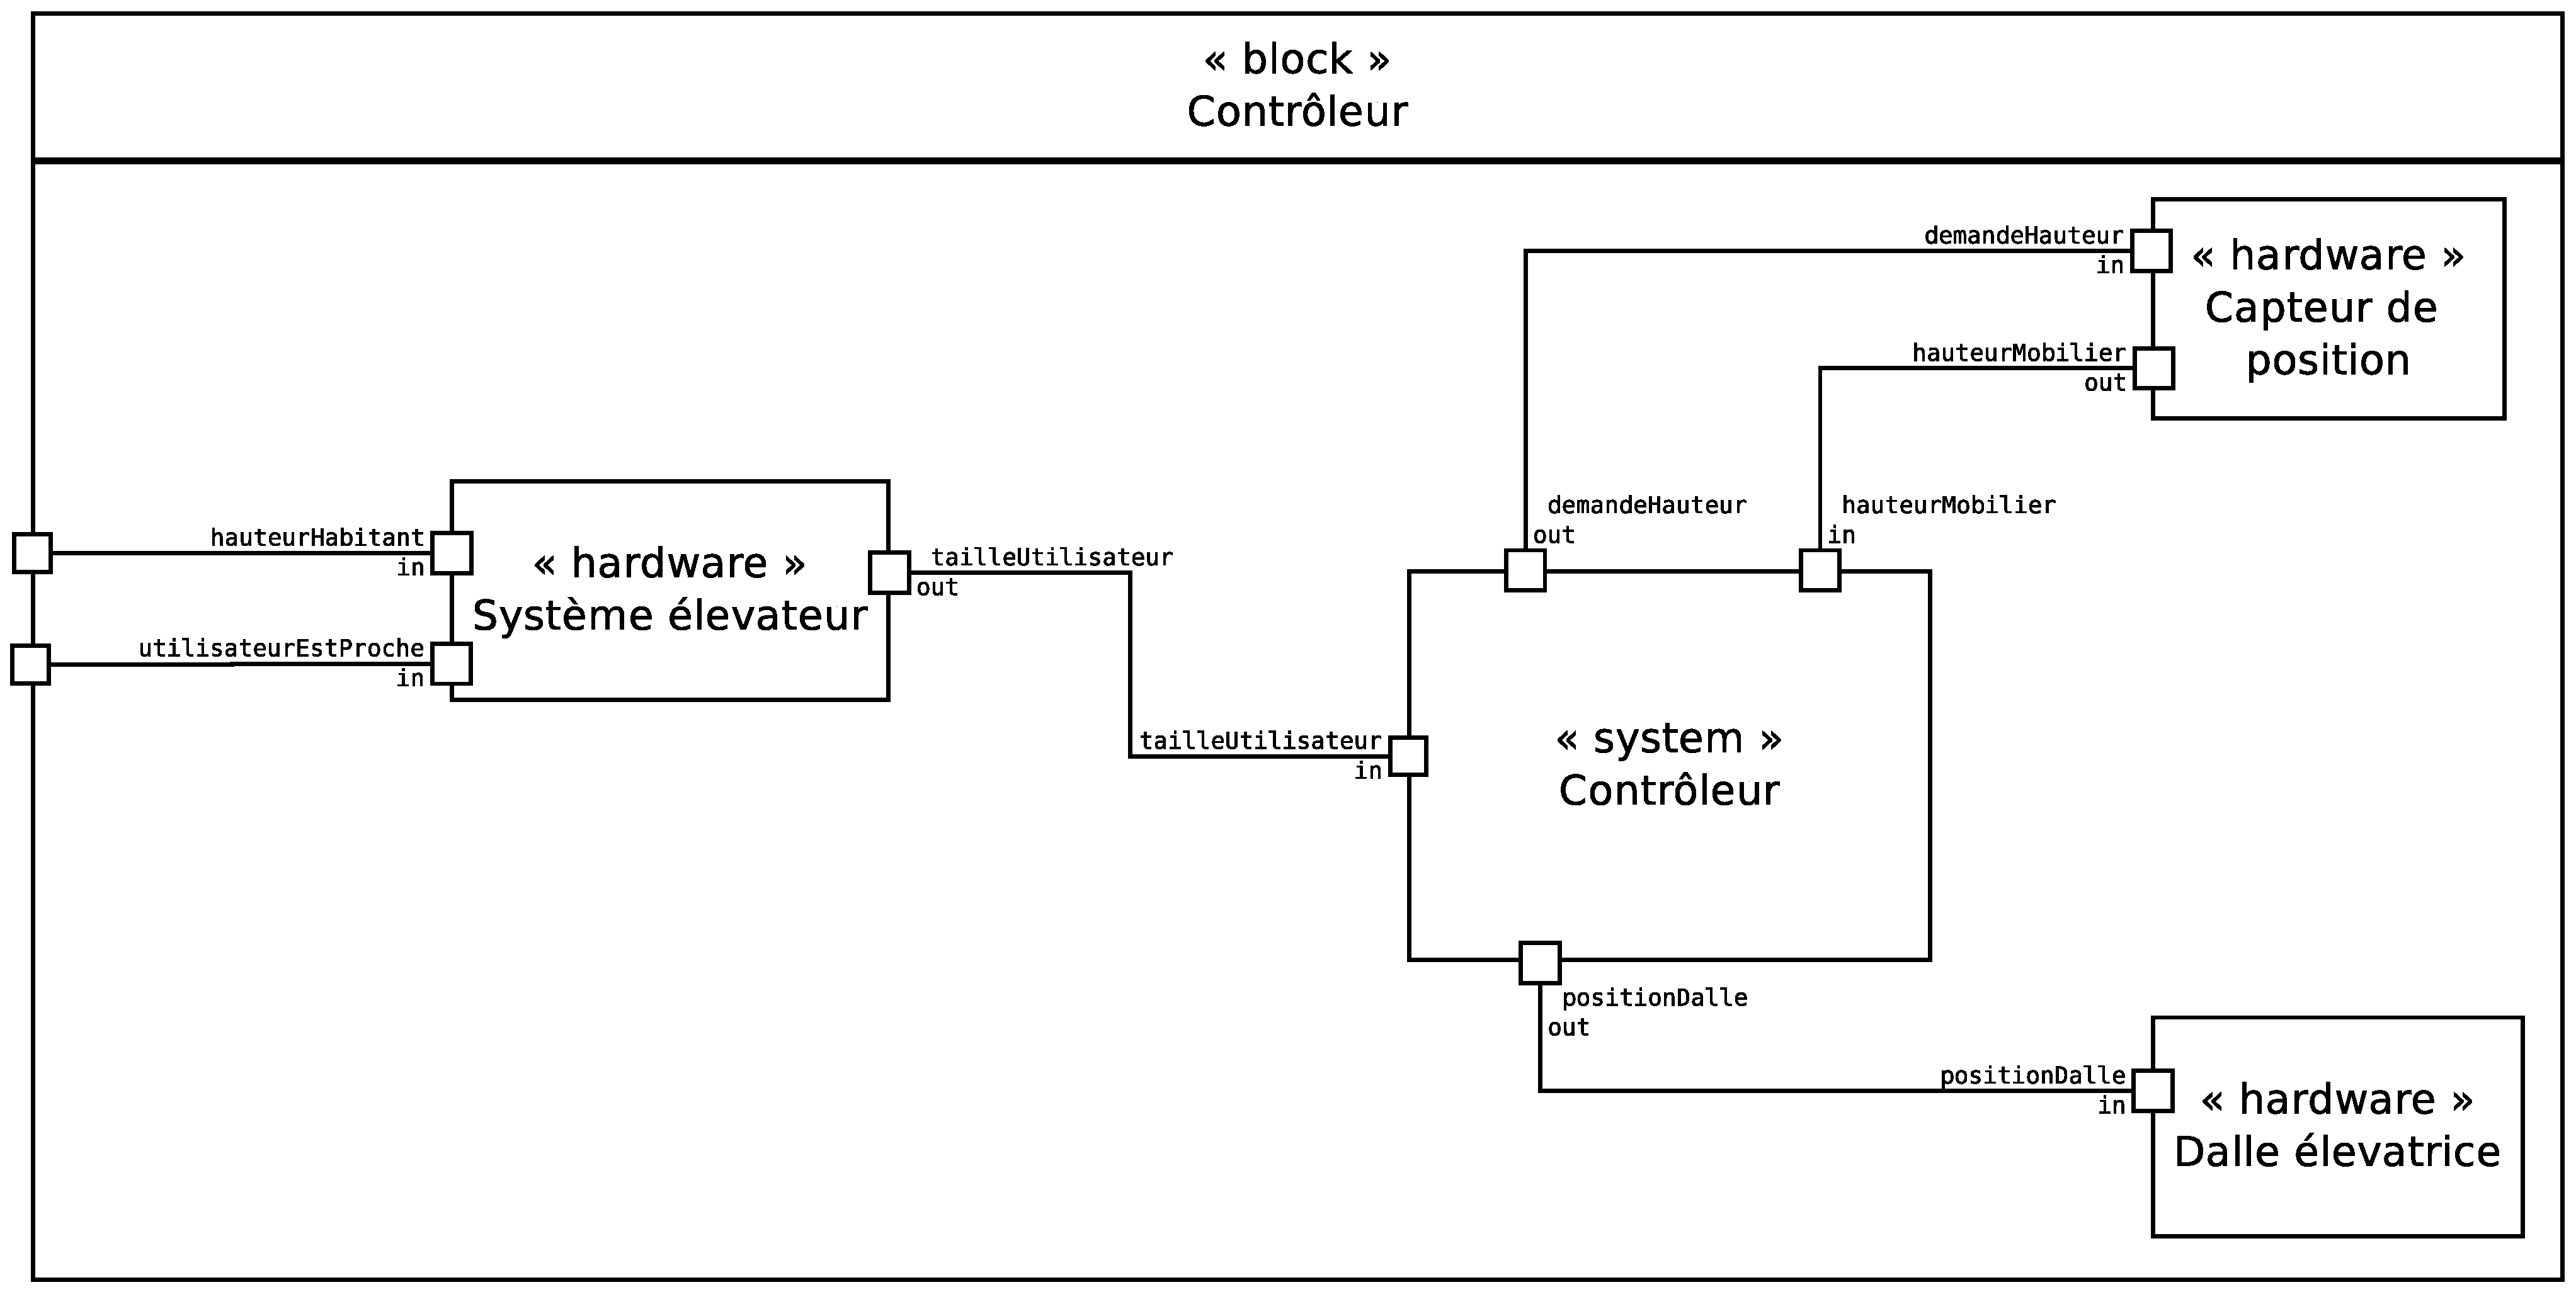
\includegraphics[width=1\linewidth]{diagrams/bathroom/diagramme_blocks_ibd.eps}
	\caption{Diagramme interne de blocs pour actionner la montée-descente d'un mobilier}
	\label{fig:diagramme_ibd}
\end{figure}
 % Diagrammes de blocks (ibd) #5
	% Diagrammes comportementaux
	\chapter{Diagrammes d'état}
\section{Diagramme d'état lors de l'entrée d'un utilisateur dans la salle de bain}
TODO
\begin{figure}[H]
	\centering
	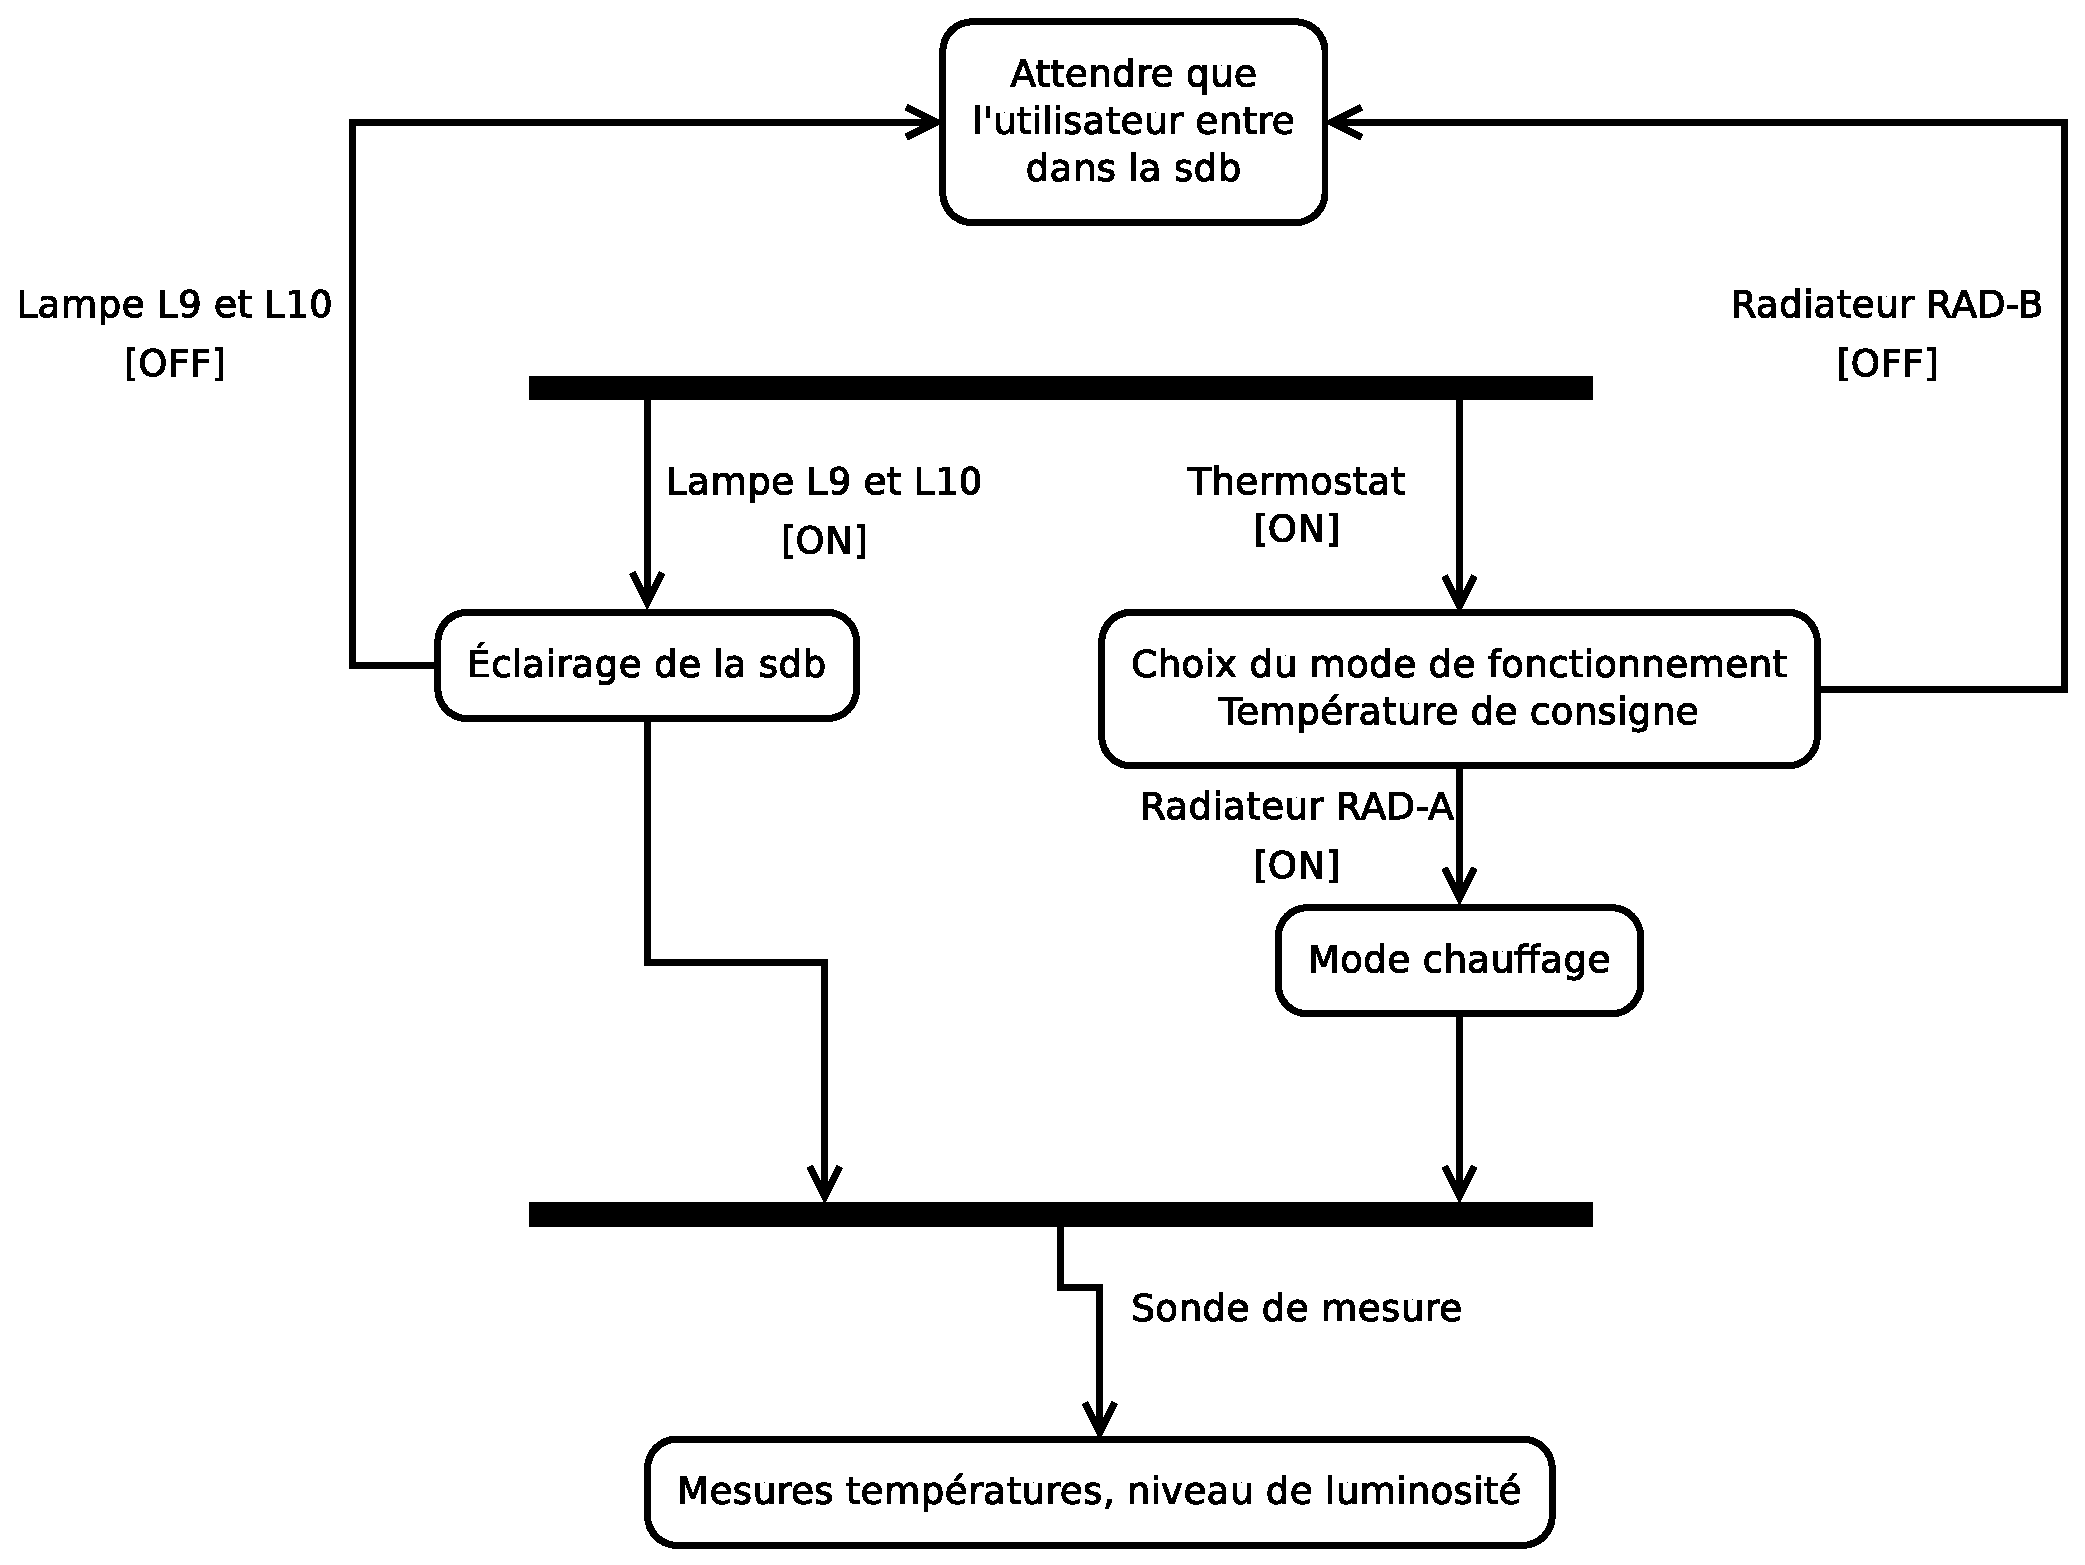
\includegraphics[width=1\linewidth]{diagrams/bathroom/diagramme_etat_st.eps}
	\caption{TODO}
	\label{fig:diagramme_st}
\end{figure}

\section{Diagramme d'état d'un utilisateur de la douche}
Le diagramme d'état ci-après décrit l'état du système lorsque l'utilisateur entre dans la douche. 

La présence de l'utilisateur dans la douche se fait au moyen d'un \textbf{capteur de charge}. Dès lors, un \textbf{capteur laser} détermine la taille de l'utilisateur afin de pouvoir adapter la hauteur de la pomme de douche à l'utilisateur. Un \textbf{capteur de position} sur le mobilier permet d'en connaître la hauteur et de la comparer à celle de l'utilisateur pour procéder à l'élévation ou l'abaissement de la dalle. 
\begin{figure}[H]
	\centering
	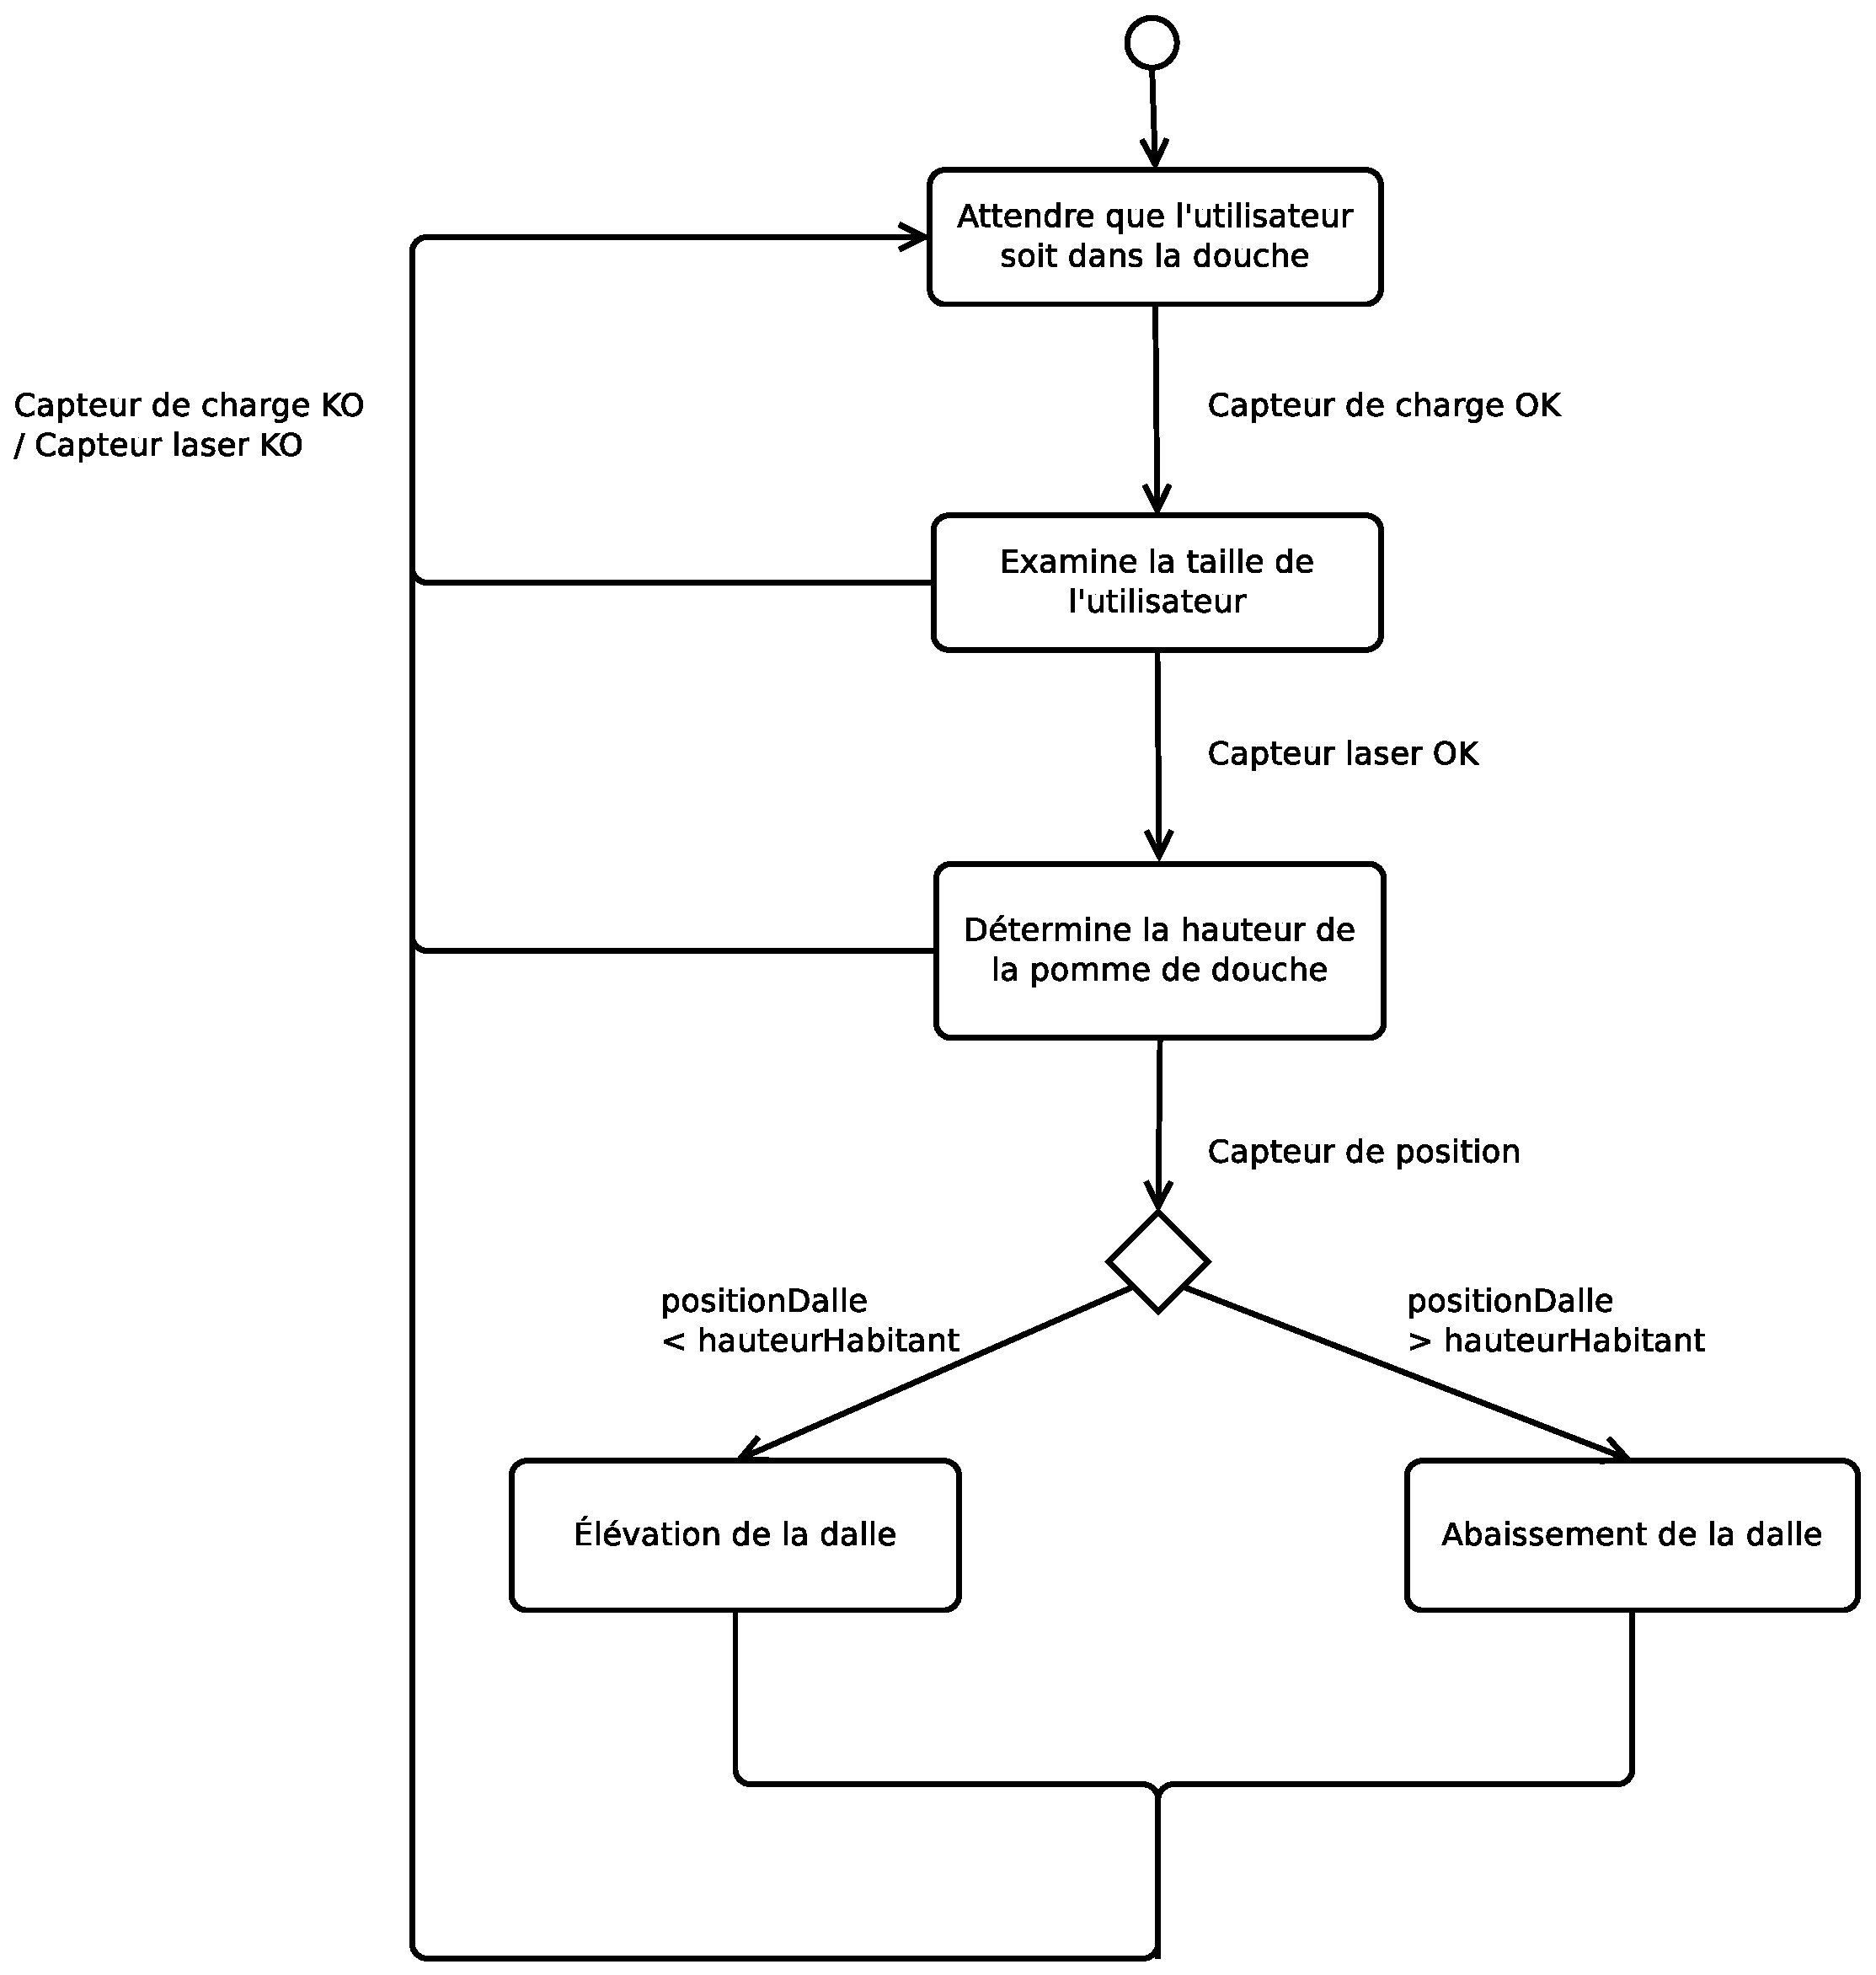
\includegraphics[width=1\linewidth]{diagrams/bathroom/diagramme_etat_st2.eps}
	\caption{Diagramme d'état d'un utilisateur de la douche}
	\label{fig:diagramme_st2}
\end{figure}
	% diagramme d'états (st) #6		
	\chapter{Diagrammes de séquence (seq)}
\section{TITRE A CHANGER 1}
%\begin{figure}[H]
%	\centering
%	\includegraphics[width=1\linewidth]{diagrams/bathroom/}
%	\caption{TODO}
%	\label{fig:diagramme_seq1}
%\end{figure}

\section{Diagramme de séquence lors de l'entré d'un utilisateur dans la douche}
TODO
\begin{figure}[H]
	\centering
	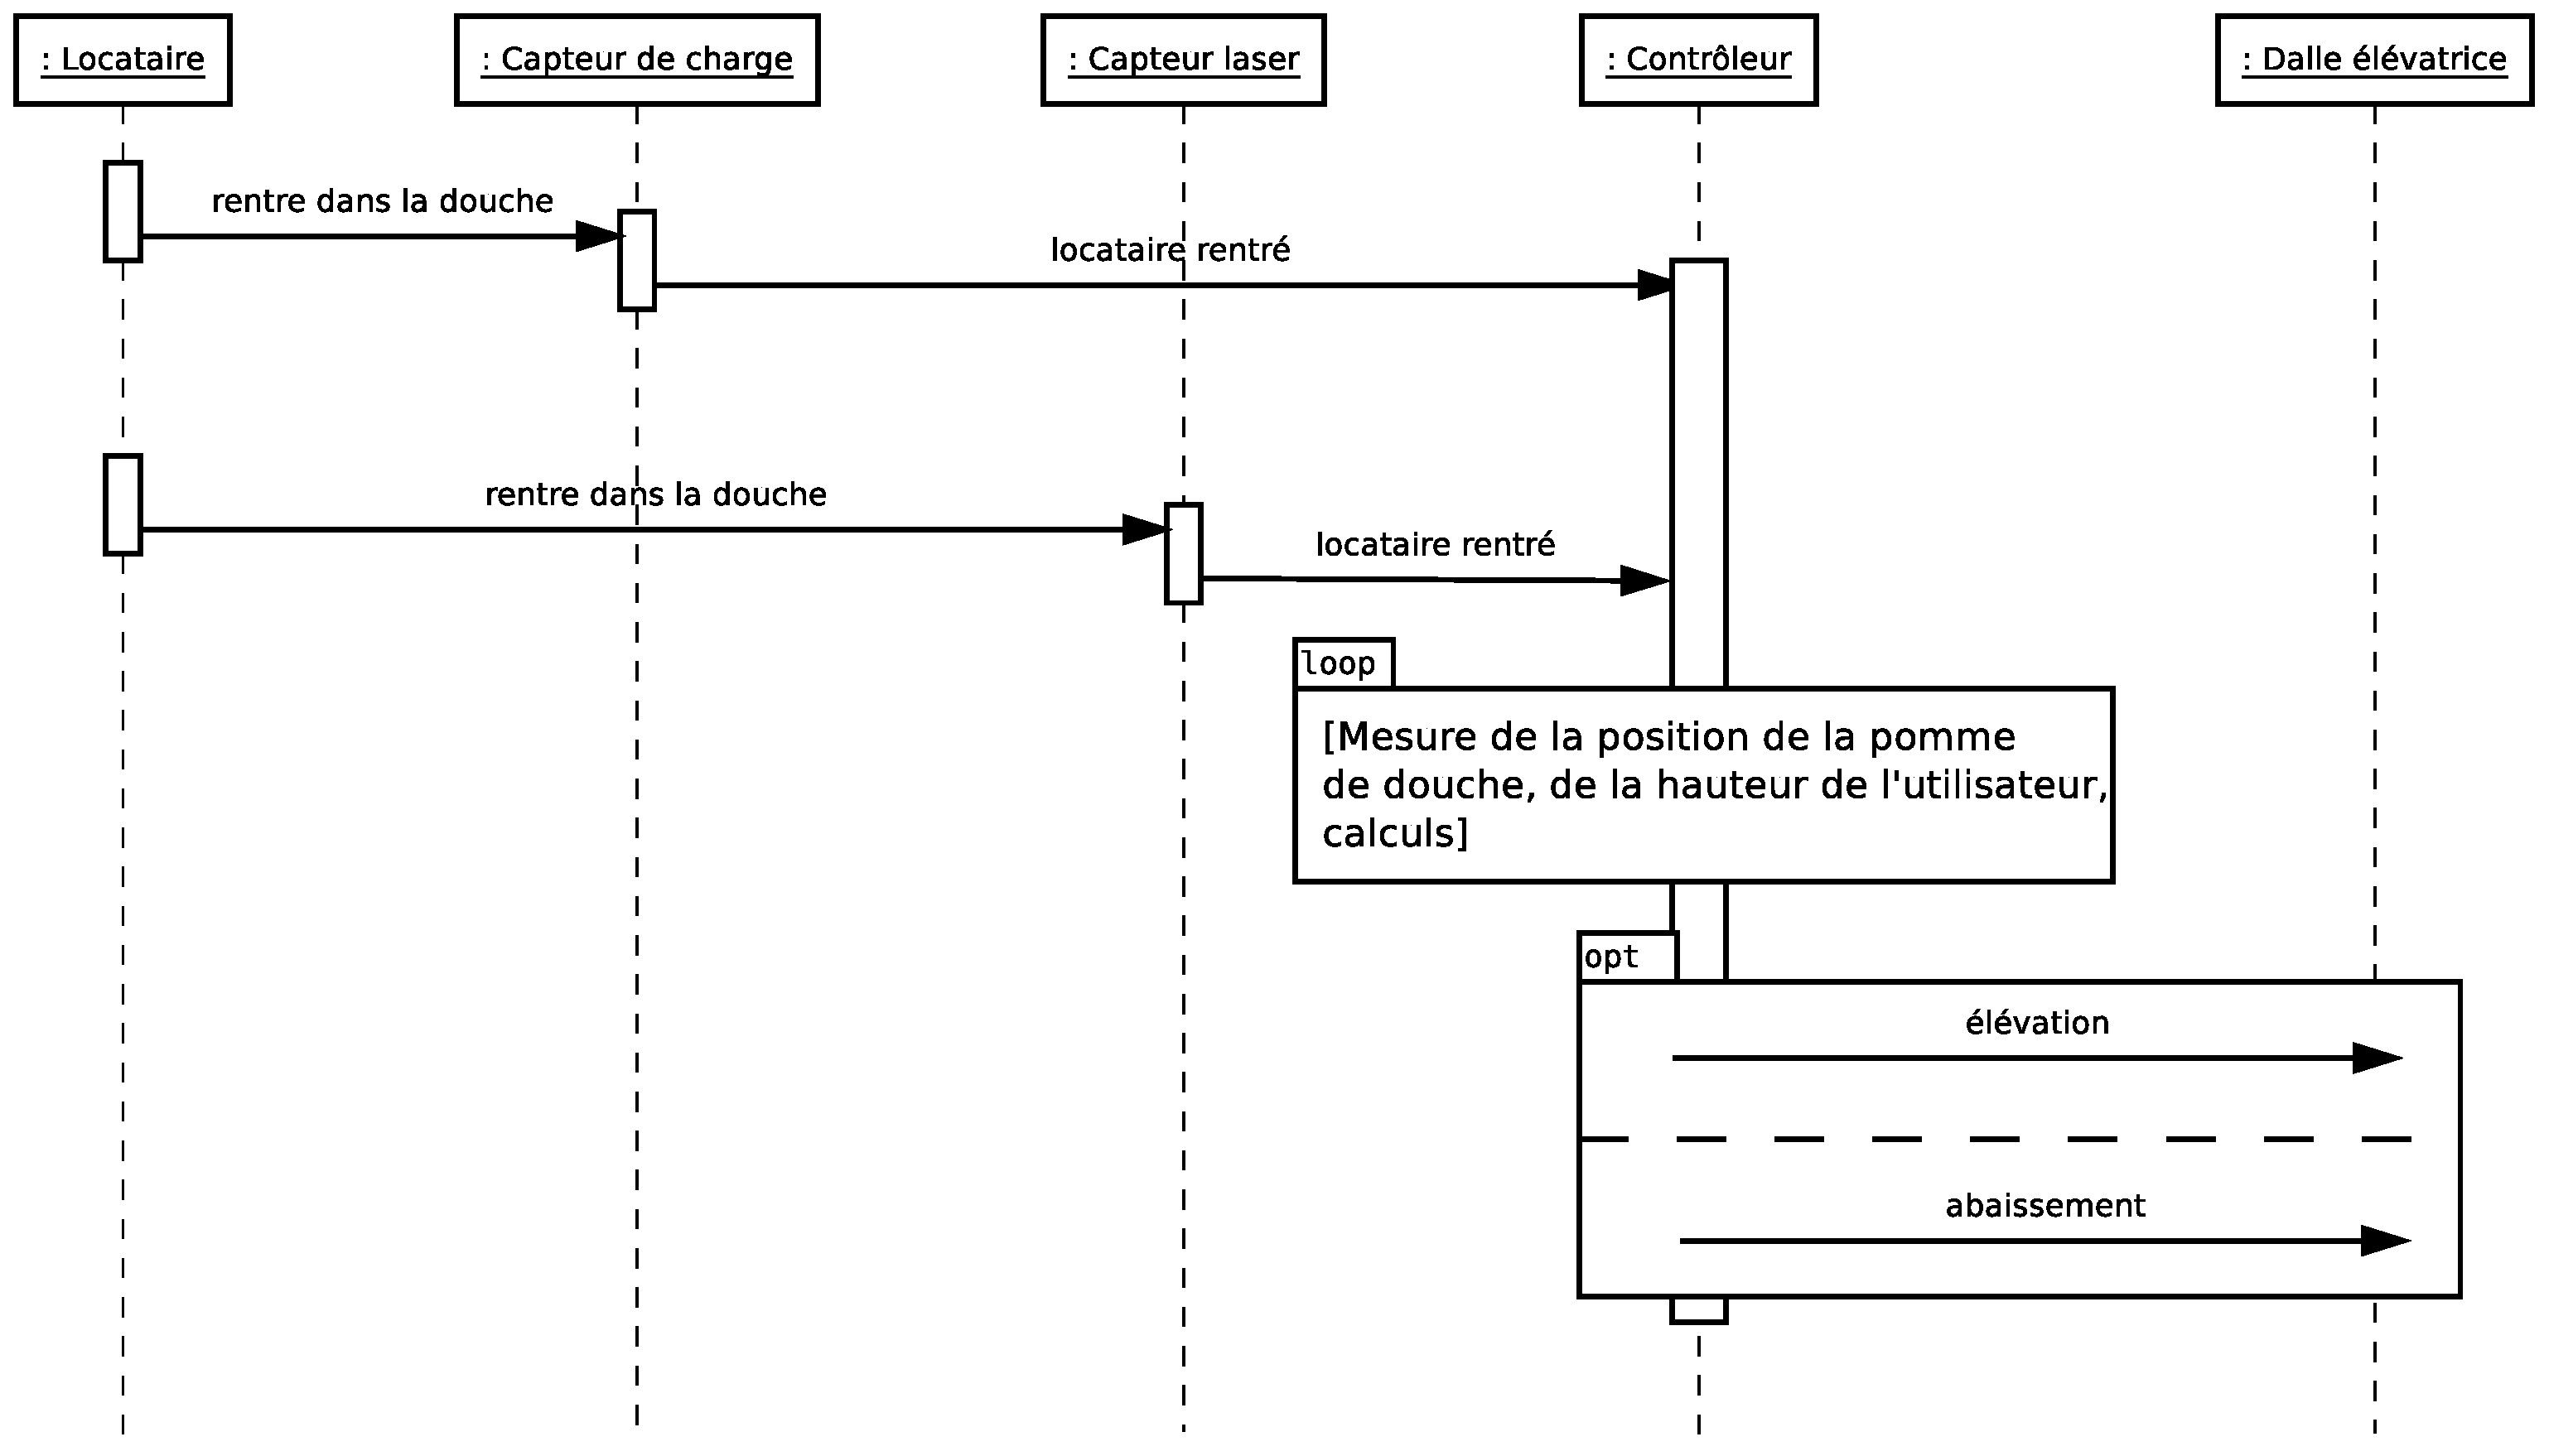
\includegraphics[width=1\linewidth]{diagrams/bathroom/diagramme_sequence2.eps}
	\caption{Diagramme de séquence lors de l'entré d'un utilisateur dans la douche}
	\label{fig:diagramme_seq2}
\end{figure}
	% diagrammes de séquences #7	

%	\chapter{Références}
\begin{description}
	\item[\Mundus~\url{http://fact-team.github.io/}] Site web de l'équipe FACT
	\item[\Mundus~\url{http://fact-team.github.io/doc/html/index.html}] Documentation \bsc{html} du projet
	\item[\Mundus~\url{https://github.com/FACT-Team/FactDev}] Code source du projet
	\item[\Mundus~\url{https://travis-ci.org/FACT-Team/FactDev}] Intégration continue du projet
	\item[\Mundus~\url{https://coveralls.io/r/FACT-Team/FactDev}] Couverture de code
	\item[\Mundus~\url{https://github.com/FACT-Team/FactDev/wiki}] Wiki de FactDev
\end{description}

	
	\listoffigures
	\printindex

\end{document}
